% !TEX TS-program = pdflatex
% !TEX encoding = UTF-8 Unicode
%\documentclass[11pt]{amsart}
\documentclass[11pt]{article} % use larger type; default would be 10pt


\usepackage{geometry} % See geometry.pdf to learn the layout options. There are lots.
\geometry{letterpaper}                   % ... or a4paper or a5paper or ... 
%\geometry{landscape}                % Activate for for rotated page geometry
%\usepackage[parfill]{parskip}    % Activate to begin paragraphs with an empty line rather than an indent
\usepackage{booktabs} % for much better looking tables
\usepackage{array} % for better arrays (eg matrices) in maths
\usepackage{paralist} % very flexible & customisable lists (eg. enumerate/itemize, etc.)
\usepackage{verbatim} % adds environment for commenting out blocks of text & for better
\usepackage{graphicx}
\usepackage{amssymb}
\usepackage{epstopdf}
\DeclareGraphicsRule{.tif}{png}{.png}{`convert #1 `dirname #1`/`basename #1 .tif`.png}

\setlength{\oddsidemargin}{-0.0in}
\setlength{\evensidemargin}{-0.0in}
\setlength{\textwidth}{6.5in}
\setlength{\topmargin}{-0.50in}
\setlength{\textheight}{9.1in}
\addtolength{\parskip}{1ex}
\setlength{\parindent}{0in}
\newcommand{\bcen}{\begin{center}}
\newcommand{\ecen}{\end{center}}
\newcommand{\lbf}{\bf\Large}
\newcommand{\lrg}{\large}
\newcommand{\nl}{\newline}
\newcommand {\z} {\vec z}
\newcommand {\p} {p_x}
\newcommand {\emx}{\epsilon_x}
\newcommand {\emy}{\epsilon_y}
\newcommand{\bit}{\begin{itemize}}
\newcommand{\eit}{\end{itemize}}
\newcommand{\sect}{\section}
\newcommand{\sub}{\subsection}
\newcommand{\bdes}{\begin{description}}
\newcommand{\edes}{\end{description}}
\newcommand{\vb}{\verb ;}
\newcommand{\bvb}{\begin{verbatim}}
\newcommand{\lan}{\langle}
\newcommand{\ran}{\rangle}
\newcommand{\benu}{\begin{enumerate}}
\newcommand{\enu}{\end{enumerate}}
\newcommand{\edoc}{\end{document}}
\newcommand{\beq}{\begin{equation}}
\newcommand{\eeq}{\end{equation}}
\newcommand{\ann}{\mbox{~~~~~and~~~~~ } }
\newcommand{\with}{\mbox{~~~~~~with~~~~~~ } }
\newcommand{\xx}{\mbox{~~} }
\begin{document}

\begin{center}  {\bf\Large Marylie Documentation Supplement: Beamline Design} \end{center}
\begin{center}  {\bf C. Thomas Mottershead }\\ 
phone: (805) 264-0583\\
email: ctmotters@gmail.com\\
\today

\ecen
\tableofcontents
\section{\bf Marylie Basics}

Marylie is a large beam dynamics and analysis code from the University of Maryland, developed by Prof. Alex Dragt and co-workers since about 1984. It uses a Lie Algebraic formulation of the transfer map, hence the name (MARYland LIE algebra). The basic theory is outlined in the LieOpticSum note. Los Alamos has been involved from almost the beginning, especially the use of the code for design purposes. This note is meant to be a brief guide for new users of Marylie for beamline design. 
%It includes supplemental documentation for the needed typecode commands, and for some new features not yet in the big manual. %The resulting master input files are ready for further analysis by Marylie 3.0 itself, as well by the parallel code Marylie-Impact.
 The current version of Marylie has some 42,000 lines of Fortran, in about 500 subroutines. It has many capabilities in beam dynamics simulation and analysis, as detailed in the 750 page user manual.

\sub{The Marylie Input File}
Marylie is driven by a master input file divided into 8 segments, each marked with a \# sign:

\vb #comment:;  Optional text describing the purpose of the present run.\\
\vb #beam   :;  Kinematic data for this run.\\
\vb #menu   :;  The pool of user defined names for instances of typecode commands\\
\vb          ;  with their associated parameters.\\   
\vb #xdata  :; Supplemental text data, alternative to external files. (new feature)\\
\vb #lines  :; Beam-lines defined by (possibly nested) sequences of user-named elements. \\
\vb #lumps  :; Instruction sequences to construct and save a map.\\
\vb #loops  :; Sequential lists of all elements in the specified lines. \\
\vb #labor  :; The program to be executed, written in the language of usernames \newline
\vb           ;defined in the other segments - \#menu, \#lines, \#loops or \#lumps.\\





\sub{TypeCodes and Keys}
 There are some 238 commands or typecodes that cause some action when invoked, typically calling a subroutine to do some calculation.  The user gives a unique name to each instance of a typecode command to be used, including its associated parameters. Sequences of these usernames in the \vb #labor; segment then serve as a program defining the calculations to be done. Unused (and unknown) typecode commands can generally be ignored. They are in five basic catagories: 
 \benu
\item  Beamline elements such as drifts, bends, and magnetic multipoles. The parameters specify their length, strength, fringe fields, etc. These compute the transfer map of the element, and concatenate it onto the accumulating working map. 
\item  Codes that make use the current map, analysing it, tracking particles through it, printing it, computing inverses, normal forms, tunes, chromaticities, etc. 
\item  Codes for adjusting the beamline element parameters to give the map desired characteristics. These design procedures are the main subject of this note.
 \item User routines that do whatever the user writes them to do, providing great flexibility. %My useful ones  are described in a section below. 
\item Random elements, user routines, and parameter sets (used for error studies).
\enu
 Appendix A has a complete list of the typecode names, with the number of parameters required for each.
The items computed from the typecode commands - map elements and measures, user routine outputs, etc. - are saved for future use, usually in a common block. There are 49 "keys" defined for reference to these computed values. Keys for array elements have associated indices. Appendix B has the full list. 


% that may be chosen as aims.
\section{Defining The Design Problem}
The design process consists of adjusting the parameters of a beamline - mainly the length and strength of the elements - to give it desired properties, e.g. $R(1,2)=0.0$ for $x$-plane focus.
Any computable characteristic of the beamline - elements of the transfer map, secondary quantities derived from it, or something computed by a user supplied subroutine - may be selected as a design aim.
The desired beamline properties are the target values $(e.g. \xx 0.0)$ for the chosen aims ($e.g. \xx R(1,2))$.

\sub{Design Aims}
 The typecode\vb `aim'; reads these aim and target definitions as text of the form:

 \vb    aim = target;

 Any number of aim and target definitions may be put on the same line, with blanks or commas as delimiters. Input is terminated by a \# sign. This text (not case sensitive) may be read from an external file, or from the new\vb #xdata; segment of the main input file. 

% A few such beamline properties are selected as design "aims", to be driven to desired "target" values  by adjusting the same number of selected beamline variables.



\sub {Internal Text Data}
The \vb #xdata; segment is a new convenience feature allowing the design process to be fully defined in the master input file. The commands\vb aim;,\vb vary;, and \vb sq; read a few lines of text defining the design aims and variables. The source is specified by their second parameter: $ p(2) = \pm N $. If $ p(2)=+N $, the source is
an external file on logical unit N. If $p(2) = -N $, the text is copied instead from block N of the \vb #xdata; segment, which has the form:
\bvb
 #xdata
     ixd>:   N1
        lines of supplemental text (e.g.  R(1,2)=0.0) for virtual unit N1
     ixd>:   N2
        more arbitrary text for virtual unit N2
\end{verbatim}
 The keyword "\vb ixd>:;" followed by a numeral N is the delimiter marking the start of virtual file N. The \vb #xdata ; block will hold up to 512 text lines, about 8 pages. The text lines may be up to 80 characters long. The virtual unit numbers (N1, N2, ...) are arbitrary, and do not need to be in sequence. Other Marylie commands may use this feature in the future.

\sub {Design Variables}
 The parameters of the defined beamline must then be adjusted to give the specified design aims their target values. Typical choices are the length or strength of selected beamline elements. 
 The typecode \vb `vary'; selects a parameter as a design variable by reading the text

\vb         username npar;

where username is the name given in \#menu to the selected element, and \vb npar; = parameter number (1 to 6) to be varied. The text is not case sensitive, and may be read from either an external file or the new \vb #xdata; segment of the main input file. Any number of variable definitions may be on the same line, delimited by blanks or commas. Input is terminated by a \# sign.

If the first parameter of \vb vary; is -1, a dependent variable may be attached to one of the primary independent variables, by entering on separate lines after the first \# sign:
\bvb
             depvar   npar
              idv    slope
\end{verbatim}
Here the first line is the username and parameter of the new dependent variable, and the second line specifies the definition sequence number (\vb idv;) of the independent variable to which it is slaved with the derivative \vb slope;. Since the number of dependent variables is otherwise unlimited, their input must always be terminated with another \# sign (or end-of-file).


For example, a Russian quadruplet made of 4 quadrupoles with usernames {\sc QA, QB, QC, QD} has the constraint that QA and QD have the same gradient with opposite signs, as do QB and QC. To maintain this symmetry while varying the two independent gradients, the \vb vary; input would be:
\bvb
      QA  2     QB  2   #
      QD  2
       1   -1.0
      QC  2
       2   -1.0
        #
\end{verbatim}
The 2 after the names selects the gradient (parameter 2) for variation. Setting \vb slope; = -1.0 insures that if QA and QD have equal and opposite gradients to begin with, that symmetry is maintained throughout the variation. QC is slaved to QB in the same manner.

%See Appendix for the\vb aim; parameter list specifying all options
\sub{Labor Iterations}
%\sub{Labor Loop}
The \vb #labor; segment is a program specifing the calulations to be done, written in the language of usernames defined in the\vb #menu; segment, with subroutines defined in the\vb #lines; segment.   
 Up to two (possibly nested) iterative processes (do loops) may be defined (eg. \vb fit,scan;).
The typecodes \vb(bip,tip); mark the begining and end of the "inner" process, and \vb(bop,top); that of the "outer". The begin points have one parameter:\vb ntimes; = the maximum iterations allowed. The number of times a loop is actually executed depends on what it contains - e.g typecode\vb fit; quits when it either converges or fails. The applicable loop number is the fifth parameter of both the \vb aim; and \vb vary; typecodes that can define independent lists of aim and variable selections for each process. 
A third list may be defined for printouts (\vb wsq;). 


% in the inner and outer for three possible uses in the \vb #labor; program:
%\benu
%\item An inner loop delimited by the \vb bip; and \vb tip; typecodes, normally used to fit targets.
%\item An outer loop delimited by the \vb bop; and \vb top; typecodes, normally used to scan a parameter.
%\item A list of aims and variables to be printed by typecode \vb wsq;.
%\enu



\section {\bf The Design Process} 
 
A point design is a location in variable space for which the computed design aims take on their target values. 

\sub{Fitting the Aims}
Marylie uses an adaptive multidimensional iterative interpolation algorithm ({\sc amdii}) to adjust the selected variables to fit the aims. The $k^{th}$ computed aim is a function $a_k({\vec x})$ on the space $\vec x$ of selected variables. A target value $t_k$ specifies a contour level hypersurface $a_k({\vec x})=t_k$ of this function. A second aim-target choice defines another such hypersurface. For a problem defined by N choices of aims, targets, and variables, we seek a common root $\vec x_r$ that zeros all the error components $f_k({\vec x_r}) \equiv a_k({\vec x_r})-t_k =0$ for $k=1,N$. This root lies in the intersection of all the contour level hypersurfaces. It may not be unique if some of the hypersurfaces are coincident. Or it may not exist if some of the hypersurfaces do not intersect.
 
The process begins with user specified feeler steps along each of the axes to compute the initial numerical derivatives. The hypersurface defined by each target equation is approximated by a hyperplane fitted to the N+1 best points so far. The process is most easily visualized in two dimesions: Each approximate plane intersects the zero plane in a line, and the crossing point of these lines is taken as the next estimate of the root. The exact functions are then recalculated at the estimated root, the new point replaces the worst previous point, and the root estimate is repeated. If all goes well, these simple multidmensional interpolation steps can rapidly converge to machine precision when they bottom out on roundoff.
 
The typecode\vb fit; does one iteration of this process. Calculation of the relevant aims must preceed it in the\vb labor; sequence. It can then update the selected variables. The first parameter is $\pm${\sc kfit}; the sign determines which loop selections to use - positive for inner, negative for outer. The other parameters specify feeler step size, error tolerance, print output, etc. See the Command Appendix for more detail.


If the new point is not the best yet, and {\sc kfit} $>1$, an interim target point is selected halfway between the real target and the best point yet, and the process restarted. This adaptive targeting may be repeated up to {\sc kfit} times to allow up to {\sc kfit-1} halvings of the reach toward the ultimate target point, rather than simply giving up on the first error increase. If the smaller step succeeds, a bigger step towards the real target is attemped. This moving target capability makes the search for a solution much more robust.


%\end{document}

\sub{Scanning the Fit}
Once an initial point design is found,
other parameters of the beamline can be scanned through a specified range to explore the response of this design point.
 Sometimes the design variables themselves may be scanned without fitting to see if the aims {\it ever} hit the targets.
%Once the design point is found, a family of similiar designs can be studied by varying other parameters not used in the fit. 
 This can be done manually, or by using the Marylie scan feature that allows any selected parameter to be incremented, and any desired inner computation repeated any number of times in an outer loop. Such parameter surveys provide clues to the range of the possible, and aid in the search for the best design, which could also need to satisfy secondary desiderata such as total length or maximum quadrupole gradients. The response of any such computable quantity to the scan parameter can be tabulated in the scan loop. An example of a Marylie file with this "scanning-the-fit" procedure is given below.

 The constraint hypersurfaces generally move with the scan parameter, and may no longer intersect beyond some limit. The final inner loop fit aims should be printed for each step of the outer scan loop to verify convergence of the fit process. In this case, any convergence failures mark the valid boundaries of the scan range.

 Convergence failures in general provide clues to the nature of the parameter space being studied. For example, if KFIT = 10 in the fit process, we are allowing up to 10 retargeting cuts. If all 10 cuts are tried, we are seeking a solution only 1/1024 the way from the current point to the original target. If even that fails, it serves as a warning that something is seriously wrong with the selection of variables and aims. Maybe there is no solution at all to the question being asked, or there is a chasm of no solution blocking the path from the initial guess to the final target. Or maybe the chosen fit variables have no effect on the chosen aims. The game is to read the convergence failures to feel out the structure of parameter space, which could require a lot of trial and error.



\subsection {Standard File Names}
One step of the design cycle may use several input and output files. These are read from or written to the fortran unit numbers specified in the typecode parameters. The choice of unit numbers and file names is actually arbitrary, but it is convenient to standardize. I give each step in the design cycle a unique case name, e.g. \vb "case";, with the Marylie input file named \vb "case.mip"; . The other associated input and output files are given the same name, with different suffixes, which can be set by a unix script. My standard file assignments were
 \bvb 
------------------------------------INPUT FILES -----------------------------
case.sca  fort.3   SCan Aims for wsq  (outer loop).    Or use ixd>:  3 in #xdata
case.ssv  fort.4   Select Scan Variables (outer loop). Or use ixd>:  4 in #xdata
case.aim  fort.7   Inner Loop Aims for fit.            Or use ixd>:  7 in #xdata
case.var  fort.8   Inner Loop Variables for fit.       Or use ixd>:  8 in #xdata
case.sq   fort.9   Select Quantities for wsq (loop 3)  Or use ixd>:  9 in #xdata
case.sv   fort.10  Select Variables  for wsq (loop 3)  Or use ixd>: 10 in #xdata
case.mip  fort.11  Marylie main InPut file
------------------------------------OUTPUT FILES -----------------------------
case.out  fort.12  Marylie main OUTput file
case.dis  fort.14  output particle set DIStribution from tracking (input on 13)
case.tmo  fort.16  Transfer Map Output file
case.next fort.17  next Marylie main input file, containing fit solution.
case.wcl  fort.20  loop contents dump
case.env  fort.24  ENVelope plot file
case.olp  fort.26  Outer Loop Print wsq (aims and variables)
case.wsq  fort.28  Write Selected Quantities (aims and variables)
case.ilp  fort.30  Inner Loop Print of aims and variables (used in fit)
case.msc  fort.34  Marylie Sine Cosine basis rays, used for Poster rayplots.
case.geom fort.35  Geometry file for Poster beamline layouts

\end{verbatim}



%\section {Appendices}




%\section {Auxilary Routines}


\sub{User Arithmetic}
Multiple calls to \vb user9; allows the construction of elaborate algebraic combinations of existing computed quantities. These new constructs can also be used as design goals. Results are available using the key \vb u(n); for the $n^{th}$ entry in \vb ucalc;.

\bit
\item There are 3 possible arithmetic operations: weighted sums, ratios, and products. 
\item The indices are used directly for the two single index quantities - Lie polynomial coefficients $f(k)$, and previously calculated ucalc entries $u(k)$.
\item The double index items such as\vb R(i,j); (R-matrix elements), and\vb tm(j,k); (Taylor map components) are handled by packing the indices: set $k = 10i+j$ to reference $R(i,j)$. 
So e.g.\vb R(1,2); would be written as $R(12)$, i.e. $k=12$. Likewise\vb tm(36,5); $(=U_{5124})$ is indexed by $k=365$ and called $T(k)$ below. 
\item All values of the constants $(a,b)$ are allowed, and they may be both stored in the\vb ucalc; buffer (for job = 0) and retrieved from it (for job = -N). This allows building more complicated formulas by repeated calls to\vb user9;.
\item Take $a=+1, b=-1$ to compute differences.
\item To store map components themselves in\vb ucalc; use $a=+1, b=0$ .
\item The following job ID sequence was chosen to be orderly with maximum backward compatibility:
\eit
%\edes
\hspace{0.8 in }\begin{tabular}{l|l|l}  %\hline
        job = -N & set job = +N and take constants from ucalc:  &  $a=u(ia)$, $b=u(ib)$  \\
        job = 0 &  store the constants in\vb ucalc; for future use:  &  $u(k) = a$, $u(m) = b$. \\
  \hline
        job = 1 & weighted sums of R-matrix elements:  &  $u(n)=aR(k)+bR(m)$  \\
        job = 2 & weighted sums of Lie coefficients: & $u(n)=af(k)+bf(m)$  \\  
        job = 3 & weighted sums of previous\vb ucalc; entries: & $u(n)=au(k)+bu(m)$ \\        
        job = 4 & weighted sums of Taylor coefficients:  & $u(n)=aT(k)+bT(m)$  \\
 \hline
        job = 5 & ratios of Lie coefficients: & $u(n)=af(k)/[b+f(m)]$  \\               
        job = 6 & ratios of Taylor coefficients: & $u(n)=aT(k)/[b+T(m)]$    \\         
        job = 7 & ratios of previous\vb ucalc; entries: & $u(n)=au(k)/[b+u(m)]$   \\                 
        job = 8 &  ratios of R-matrix elements: & $u(n)=aR(k)/[b+R(m)]$  \\ 
\hline            
        job = 9 &  products of Lie coefficients: & $u(n)=af(k)[b+f(m)]$ \\                
        job = 10 &  products of Taylor coefficients: & $u(n)=aT(k)[b+T(m)]$  \\           
        job = 11 &  products of previous\vb ucalc; entries: & $u(n)=au(k)[b+u(m)]$     \\              
         job = 12 &  products of R-matrix elements: & $u(n)=aR(k)[b+R(m)]$   \\  
\hline        
        job = 13 &  RMS of the two ucalc entries: &  $u(n)=\sqrt{u(k)^2+u(m)^2}$ \\
        job = 14 &  reciprocal of variable k in selection loop m: & $u(n)=1/x(k,m)$ \\
%\hline
\end{tabular}
%\end{document}
%\edoc



%\edoc

\section{Example: Focusing a Magnifier}
This Marylie input file example (\vb rqmag.mip;) focuses a 3X magnifier in both planes. The quadrupole gradients in \vb #menu; are initial guesses. The \vb next; command after the fit writes a  copy of this master file containing the new fitted values, for future use. Text after an exclamation point is a comment.
\bvb
 #comment
  Russian Quadruplet Magnifier Focus Example.  23 GeV protons.                 
   Mass =  938.2796   K.E.=    23000.0000 Mev   P=    23.919877 Mev/c          
   Charge=  1.     Brho =   79.78812 Tesla-meters                              
   Beta (v/c)= 0.99923156   Gamma=    25.513147   Eta=    25.493542            
 #beam   
   79.788121020000006     
   24.513147629999999     
   1.0000000000000000     
   1.0000000000000000     
 #menu   
  next     pmif
    1    17    2      
  clear    iden    
  begin    bip     
    1000
  endfit   tip     
     0   
  beamin   usr8
   0.01  0.0   0.002  0.01  0.0   0.002   ! 1 cm X 2mrad beam
  aim      aim 
    2   -7   0    1    1    3    ! select  aims from    ixd>:  7   
  vary     vary 
   -1   -8   0   0   1   3      ! select  variables from ixd>: 8
  fit      fit 
   10    0    0   0.02   0   3        
  qa       quad                        !
   0.6     50.0      1.0   1.0      ! 
  qb       quad                        !   Initial guesses
  0.9     -60.0      1.0   1.0     !
  qc       quad                        !
   0.9      60.0     1.0   1.0     !
  qd       quad                       !
   0.6     -50.0     1.0   1.0    !  
  focal    drft    
    1.0  
  throw    drft                       ! Long final drift
    9.0
  gap      drft    
   0.6   
  center   drft    
    1.4  
  mapsav   tmo     
    16   
  linout   usr1
    1   1   20   1    3    0     
  aper     ps9
   0.01   0  0  0  0  0    
  fin      end     
 #xdata  
  ixd>:  7
      R(1,2)=0.0  R(3,4) = 0.0  R(1,1) = -3.0 #     ! x and y focus, with -3X magnification                           
  ixd>:  8
        qa  2   qb  2  throw 1 #     ! Vary Russian Quadruole Gradients, and final drift                                               
        qd  2                                                                           
        1  -1.0                                                                    
        qc  2                                                                           
        2  -1.0                                                                         
        #                                                                               
 #lines    !a Russian quadruplet magnifier
  russ    
      1*aper        1*focal       1*qa          1*gap         1*qb       &
      1*center      1*qc          1*gap         1*qd          1*focal    &
      1*throw   
 #lumps  
 #loops  ! Unroll the full layout
  layout  
      1*russ    
 #labor  
     1*clear  ! clear the buffers
     1*russ   ! compute initial map
     1*aim    ! select aims 
     1*vary   ! select variables 
     1*begin  ! start of inner loop 
     1*clear  ! clear the map
     1*russ   ! compute map of line
     1*fit    ! update variables
     1*endfit ! end of inner loop 
     1*next   ! save the results. If you are here, the fit loop is finished
     1*clear  ! start over
     1*russ   ! compute final map
     1*mapsav ! save it to file 16
     1*beamin ! choose input beam moments
     1*layout ! expand the line
     1*linout ! report final design
     1*fin    ! all done 
\end{verbatim} 

\sub{Resulting Output}
File \vb rqmag.out;: First echo the aims, variables and targets. Then do 16 fit iterations that bounce off the bottom (machine precision). Quit on first error increase below $10^{-9}$, and report final fitted beamline and resulting output beam. No target cuts were needed. Convergence was easy.
\bvb
Marylie 2014 version with #xdata
           7  lines read into mltext common.
  1: id=  7  R(1,2)=0.0  R(3,4) = 0.0  R(1,1) = -3.0 #                                       
  2: id=  8  qa  2   qb  2  throw 1 #                                                        
  3: id=  8  qd  2                                                                           
  4: id=  8  1  -1.0                                                                         
  5: id=  8  qc  2                                                                           
  6: id=  8  2  -1.0                                                                         
  7: id=  8  #                                                                               
  
  Aims selected : 
 No.     item        present value        target value
-----------------------------------------------------
  1    r(1,2) =      -1.61645789          0.00000000    
  2    r(3,4) =       1.13230270          0.00000000    
  3    r(1,1) =      -2.70692910         -3.00000000    

   Variable #menu elements selected:
 No.  Element    Type     Parameter   Present value.
------------------------------------------------------------
  1    qa         quad         2       50.000000000000    
  2    qb         quad         2      -60.000000000000    
  3    throw      drft         1       9.0000000000000    

   Dependent #menu elements selected:
 No.  Element    Type     Parameter   Present value       IDV  Slope
------------------------------------------------------------------------
  1   qd         quad       2      -50.000000000000        1  -1.00000
  2   qc         quad       2       60.000000000000        2  -1.00000
 Iter   1 Error= 1.6165E+00,  Step= 1.0000E+00,  SubErr= 1.6165E+00 @cut=    1
 -------------------------------------------------------
                    :
                    :
 -------------------------------------------------------
 Iter  15 Error= 2.2204E-15,  Step= 7.1607E-15,  SubErr= 2.2204E-15 @cut=    1
 -------------------------------------------------------
          16 = iter final value.
 Quit on iteration    16 for reason 2: Best effort: Hit bottom at full reach   
 Final values with reach =    1 are:
  
  Aims selected : 
 No.     item        present value        target value
-----------------------------------------------------
  1    r(1,2) =      2.220446049E-15      0.00000000    
  2    r(3,4) =       0.00000000          0.00000000    
  3    r(1,1) =      -3.00000000         -3.00000000    
  
  New values for parameters:
 No.  Element    Type   Parameter   Present value         IDV  Slope
------------------------------------------------------------------------
  1   qa         quad       2       54.299888446587    
  2   qb         quad       2      -59.244687227295    
  3   throw      drft       1       9.9915286067318    
  4   qd         quad       2      -54.299888446587        1   -1.0000
  5   qc         quad       2       59.244687227295        2   -1.0000
  
  Maximum error is     2.220446E-15
  Maximum allowed was   0.00000    

 
  Line has   6 drifts and   4 quads
  Beam Line Summary
   n  name     type   aper[cm] length[cm]    Gradient     PoleTip[g]   path[cm]
   1  focal    drift    1.00   100.000      0.0000000        0.00000   100.000
   2  qa        quad    1.00    60.000     54.2998884     5429.98884   160.000
   3  gap      drift    1.00    60.000      0.0000000        0.00000   220.000
   4  qb        quad    1.00    90.000    -59.2446872    -5924.46872   310.000
   5  center   drift    1.00   140.000      0.0000000        0.00000   450.000
   6  qc        quad    1.00    90.000     59.2446872     5924.46872   540.000
   7  gap      drift    1.00    60.000      0.0000000        0.00000   600.000
   8  qd        quad    1.00    60.000    -54.2998884    -5429.98884   660.000
   9  focal    drift    1.00   100.000      0.0000000        0.00000   760.000
  10  throw    drift    1.00   999.153      0.0000000        0.00000  1759.153
 Total length =        17.59153[m],  Sum|GL| =   171.800303[T]
\end{verbatim}
\sect{Beamline Rayplot Checks} 
A first order rayplot is a useful check on the solution just found, especially to verify that it is a ground state solution rather than an excited state. This uses \vb user1 ; to generate the sinelike and cosinelike basis rays (Dave Carey's notation), and a graphics package like {\sc poster} to plot them.
% It can also propagate basis rays and the $\sigma$ matrix through the slices to write files that {\sc poster} can use for ray and envelope plots. The current best (somewhat evolved) procedure is:
\sub{Generating Basis Functions}
To generate basis rays, put the beamline in a \vb #loop; to unroll any included lines to a flat array. With this named loop in the \vb #labor; segment, run Marylie \vb usr1; to slice the drifts and quadrupoles and generate a file of basis rays for the beam line of interest.
So far this can only be a sequence of drifts, quads, and aperture settings.
    The aperture is taken to be p(1) of PS9 (Parameter Set 9), and applies to all
    following elements until reset by another aperture command
 Save on fort.34, renamed to case.msc (MarylieSineCosine).
 The {\sc usr1} parameters should be:
\benu
\item{\sc job} = 1 to slice the elements and fill in the sincos buffer for future use.
\item{\sc menv} = 1 to write the sincos buffer to the .MSC file (lun=34)
\item{\sc mincut} = minimum no. of slices/element (at least 7 slices for short elements like quads.)
\item{\sc step} = nominal thickness of one slice. First try nslice=length/step, but it
                  must be at least mincut. Actual final dz = length/nslice.
\item{\sc isend} = 3 as usual for both jof and jodf output.
\item{\sc jtran} = 0 for no translation files (unused option).
\enu


  Content of the resulting .MSC file:
	
	\vb line 1;= {\sc nep, nflg, wx, wy, brho, beta, gamm1}:, where

	 {\sc nep}  = points needed to draw quad blocks,  {\sc nflg} = 0 is not used,
{\sc (wx,wy)} are the x,y achromatic correlation coefficients, and {\sc brho,beta,gamm1} are the usual kinematic parameters.

   \vb lines 2,nep+1; = z, radius, G[T/M], n, typecode, name = beamline data  \newline (at each element edge) for drawing quadrupole boxes

	\vb lines nep+2,EOF; :  z,r,cx,sx,cy,sy: cosine and sine basis rays at each z-point. 

The achromatic correlation coeffients are computed from the Taylor map terms \newline
{\sc wx} = -tumat(12,1)/tumat(17,1) and \newline
{\sc wy} = -tumat(21,3)/tumat(24,3)      


%\edes 
%\end{document}
============================================================
\sub{{\sc poster} Ray Plots}

{\sc poster} is a script driven program to generate PostScript plots from a variety of data types. The Mac OS displays PS plost as pdf's, which may be saved for inclusion in documents like this one. Appendix C lists all of the commands. The followng script sets plot scales, 
loads color tables, specifies number and spacing of rays in both position and angle, and draws the ray plot:
 \bvb
#page 1  6 606 360  782 .75 0.75  0  0 
 #font  Helvetica
 #text Pathlength [m]
  0 0 0  300  380 0 14 0
 #area  81  574  421  720  1  3030  10  1
   0 0.0 
17.60 -2.5  2.5  2 1 0 0
 #font Helvetica
 #text  Russian Quadrupole 3X Magnifier, 23 Gev/c protons.
  0 0 1 150  740 0 16 0
 #text Transverse position [cm]
  0 0 0  40 600  90 14 0
 #bbox
 #load 6 0.5 0.5             ! load 6 colors
 dot 1 0  1  1 0 2.5  20  0 0 0
 dot 2 0  1  1 0 2.5  20  0 0.7  0.0
 dot 3 0  1  1 0 2.5  20  1 0 0
 dot 4 0  1  1 0 2.5  20  0 0 1
 dot 5 0  1  1 0 2.5  20  0.5 0.4 0.0
 dot 6 0  1  3 0 1.5  20  1.0 0.9 0.7
 #rays  #file RQMag.msc
 2  4  2 1 -6 0.40 0.25  !    nrl,  nsa,  job,  ka,   kb,  delta,  dphi
 #text x-plane rays
 5 1 20 285 710 0 10 12
 0.00 mR
 0.25 mR
 0.50 mR
 0.75 mR
 1.00 mR
---------------------------------------------------------
Parameters:
         Rays to generate:
            nrl  = no. of ray locations to generate (on each side of axis)
            nsa  = no. of scattering angles to generate (each side of zero)
            job = 2 to generate achromatic rays using (wx,wy) from .msc file.
            job = 3 to generate plain uncorrelated rays (wx = wy = 0.0)
              signs: If job > 0 use same color key for both signs of scattering.
                        If job < 0 use next color key for negative scattering angles.
         View plane:
            ka = 1 for x-axis,
            ka = 2 for y-axis
         Quad box flag:
            kb = 0 for none,
            kb = +K for inside boxes, where K=color key to use for the box.
            kb = -K for outside boxes.(K is skipped for the ray color sequence.)
         Ray steps:
            delta= position step in [cm]
            dphi = scattering angle step [mR]
\end{verbatim}  
    
\begin{figure}[ht!] 
{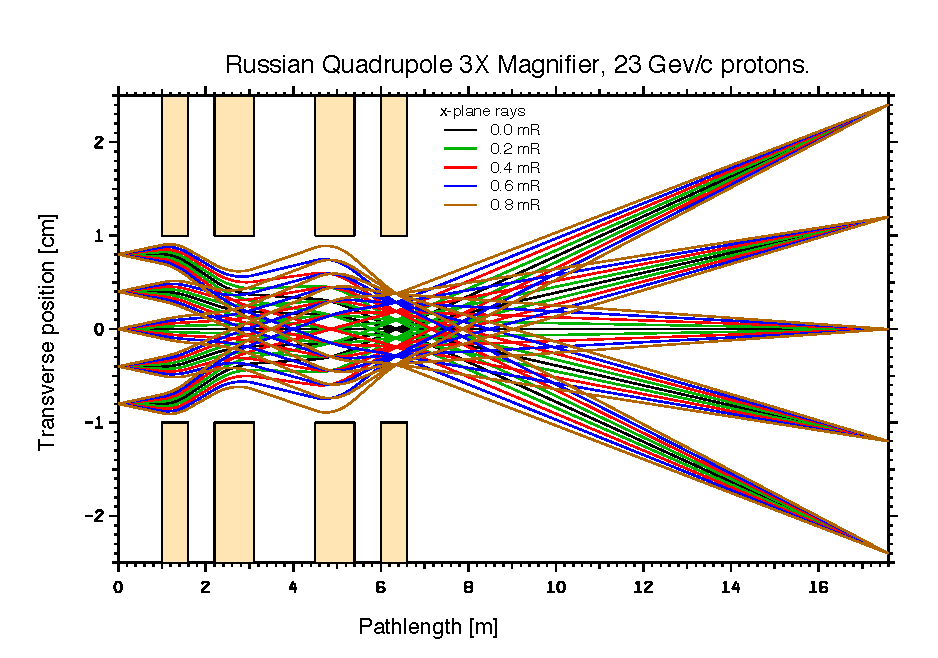
\includegraphics[width=6.0in]{RQMag.pdf}}
\caption{ Russian Quadruplet Magnifier }
\end{figure}

\newpage
\section{Appendices}
\sub {A: All Typecodes}

The 238 typecodes and number of required parameters. Chapter 13 of the big manual lists the purpose of each typecode, with references to more complete documentation. The 53 randomized variants are for error studies.
\bvb
Group 1 <---------  34 typecodes for beamline elements:---------->
  1  drft      6  nbnd      4  pbnd      6  gbnd      2  prot
  4  gbdy      5  frng      6  cfbd      4  quad      2  sext
  2  octm      2  octe      2  srfc      1  arot      4  twsm
  6  thlm      5  cplm      4  cfqd      5  dism      6  sol
  0  mark      0  jmap      0  dp        6  recm      1  spce
  4  cfrn      6  coil      6  intg      6  rmap      4  arc
  6  sbnd      4  rbnd      6  gmag      9  gendip
Group 2 <---------  20 typecodes for user routines:-------------->
  6  usr1      6  usr2      6  usr3      6  usr4      6  usr5
  6  usr6      6  usr7      6  usr8      6  usr9      6  usr10
  6  usr11     6  usr12     6  usr13     6  usr14     6  usr15
  6  usr16     6  usr17     6  usr18     6  usr19     6  usr20
Group 3 <---------   9 typecodes for parameter sets:------------->
  6  ps1       6  ps2       6  ps3       6  ps4       6  ps5
  6  ps6       6  ps7       6  ps8       6  ps9
Group 4 <---------  24 typecodes for randomized elements:-------->
  2  rdrft     2  rnbnd     2  rpbnd     2  rgbnd     2  rprot
  2  rgbdy     2  rfrng     2  rcfbd     2  rquad     2  rsext
  2  roctm     2  rocte     2  rsrfc     2  rarot     2  rtwsm
  2  rthlm     2  rcplm     2  rcfqd     2  rdism     2  rsol
  2  dummark   2  dumjmap   2  dumdp     2  rrecm
Group 5 <---------  20 typecodes for randomized user routines:--->
  2  rusr1     2  rusr2     2  rusr3     2  rusr4     2  rusr5
  2  rusr6     2  rusr7     2  rusr8     2  rusr9     2  rusr10
  2  rusr11    2  rusr12    2  rusr13    2  rusr14    2  rusr15
  2  rusr16    2  rusr17    2  rusr18    2  rusr19    2  rusr20
Group 6 <---------   9 typecodes for randomized parameter sets:-->
  2  rps1      2  rps2      2  rps3      2  rps4      2  rps5
  2  rps6      2  rps7      2  rps8      2  rps9
Group 7 <---------  43 typecodes for map utilities:-------------->
  6  rt        0  sqr       2  symp      4  tmi       1  tmo
  3  pmif      6  circ      1  stm       2  gtm       0  end
  5  ptm       0  iden      2  whst      0  inv       0  tran
  1  revf      0  rev       6  mask      5  num       4  rapt
  2  eapt      6  of        6  cf        5  wnd       6  wnda
  4  ftm       2  wps       3  time      1  cdf       0  bell
  2  wmrt      3  wcl       0  paws      5  inf       6  dims
  4  zer       4  wuca      6  tpol      5  dpol      6  cbm
  1  pli       2  wexa      3  shoa
Group 8 <---------  42 typecodes for map analysis:--------------->
  6  cod       6  amap      5  dia       5  dnor      3  exp
  5  pdnf      5  psnf      4  radm      4  rasm      5  sia
  5  snor      5  tadm      6  tasm      1  tbas      2  gbuf
  6  trsa      6  trda      3  smul      5  padd      3  pmul
  3  pb        5  pold      4  pval      6  fasm      6  fadm
  4  sq        6  wsq       4  ctr       6  asni      4  pnlp
  1  csym      3  psp       2  mn        6  bgen      6  tic
  6  ppa       6  moma      6  geom      3  fwa       4  merf
  3  lnf       0  taylor
Group 9 <---------  37 typecodes for beamline design:------------>
  1  bip       1  bop       1  tip       1  top       6  aim
  6  vary      6  fit       6  opt       6  con1      6  con2
  6  con3      6  con4      6  con5      2  mrt0      6  mrt1
  6  mrt2      6  mrt3      6  mrt4      6  mrt5      1  fps
  6  cps1      6  cps2      6  cps3      6  cps4      6  cps5
  6  cps6      6  cps7      6  cps8      6  cps9      4  dapt
  6  grad      5  rset      6  flag      6  scan      6  mss
  3  cxp       2  tqm

\end{verbatim}


\sub{B: All Keys to Possible Aims}
% The symbols are made of two character keywords, some with associated indices. Some 49 of them are defined for standard computed quantities in Marylie: 

The standard computed quantities that may be chosen as possible design aims are labeled by  49 two letter "keys", some with associated indices:
\bvb 
      data key/
     $'sm', 'bm', 'sf', 'bf', 'ba', 'tn', 'tp', 'en', 'r(', 'z(',
     $'d(', 'tm', 'ex', 'f(', 'u(', 'um', 'ls',
     $'tx', 'ty', 'ts', 'cx', 'cy', 'qx', 'qy', 'hh', 'vv', 'tt',
     $'hv', 'ht', 'vt', 'fx', 'xb', 'xa', 'xu', 'xd', 'fy', 'yb',
     $'ya', 'yu', 'yd', 'pl', 'rt', 'st', 'ek', 'pd', 'br', 'be',
     $'ga', 'gm'/
\end{verbatim} 
\benu
\item    Array Components
  \bvb
  Current Map
     r(i,j)  : First order (linear) matrix elements i,j=1,6.
     f(i)    : Lie polynomial coefficients, i=1,209.
     tm(i,jg): Taylor expansion coefficients, i=1,6, jg = Georgelli index    
  Stored Maps
     sm1(i,j) ... sm5(i,j) :  First order (linear) matrix elements i,j=1,6.
     sf1(i) ...   sf5(i)   :  Lie polynomial coefficients, i=1,209.
  Work Buffers
     bm1(i,j) ... bm5(i,j) :  First order (linear) matrix elements i,j=1,6.
     bf1(i) ...   bf5(i)   :  Lie polynomial coefficients, i=1,209.
 \end{verbatim}
\item  Characteristics of the current map: tunes, chromaticities,
       anharmonicities, dispersions, and twiss parameters.
\bvb
  Tunes:  (call TASM)
     tx, ty = horizontal and vertical tunes.
         ts = synchrotron (temporal) tune for a dynamic map,
              or temporal dispersion (eta) for a static map.
  Chromaticities:
     cx, cy = horizontal and vertical 1st order chromaticities.
     qx, qy = horizontal and vertical 2nd order (quadratic) chromaticities.
  Anharmonicities:
     hh, vv, tt, hv, ht, vt = second order anharmonicities.
  Dispersions:
     dz1, dz2, dz3, dz4 = first order dispersions for the
                          transverse phase space coordinates.
  Twiss parameters (zeroth order):
     ax,bx,gx = horizontal alpha, beta, gamma.
     ay,by,gy = vertical alpha, beta, gamma.
     at,bt,gt = temporal alpha, beta, gamma.
  Principal Planes Analysis (call PPA)
      (t-plane not yet implemented)
     xu, yu, tu = distance to upstream focal point for (x,y,t) planes
     xd, yd, td = distance to downstream focal point for (x,y,t) planes
     fx, fy, ft = equivalent focal lengths for (x,y,t) planes
     xb, yb, tb = drift before thin lens for (x,y,t) planes
     xa, ya, ta = drift after thin lens for (x,y,t) planes
\end{verbatim}
 \item     Beam Properties.
\bvb
  Beam Coordinates:
     z(i,j) = jth coordinate (j=1,6) of ith particle (i=1,nrays)
  Moments computed by AMAP:
     s(i,j) = 2nd moments of the beam <zi,zj>.
     bf1(i) = moments of the beam in standard Lie monomial sequence.
  Emittances:
     ex,ey,et = rms emittances for the x, y, and t planes.
     wx,wy,wt = eigen emittances for coupled systems.
\end{verbatim}
 \item  User Computed Quantities   
   \bvb
     u(i) = ucalc(i), i=1,1024. (from usr1 ... usr20)
     um1 ... um5 = user provided merit functions.
 \end{verbatim}
 \enu



\subsection{C: All {\sc poster} Commands}

%\subsection{Setup} These set parameters that are valid until replaced by another call to the same command:
\begin{description}
  \item[\#arcs] - draw arcs specified by pathlength, bend angle, and style key.                                                 
  \item[\#area]  - define the plot area in  the page, and map data coordinates to it. Draw axes.              
  \item[\#arrow] - draw an arrow.                                                                                               
  \item[\#autocad] - also write final coordinates to external files in {\sc autocad} format.                                    
  \item[\#axis] - draw axes on current plot area (use to put axes on top layer).                                                
  \item[\#bbox]  - draw thin line just outside the EPS bounding box.                                                            
  \item[\#color] - load image pseudocolor lookup table for subsequent images.                                                   
  \item[\#cols] - plot y-profile = selected column average of current image.                                                    
  \item[\#contour] - draw contour plot of 2D data.                                                                              
  \item[\#data] - main curve plotting command. get $(x,y)$ data from specified data file, or inline.                                
  \item[\#draw] - draw a simple inline x-y  plot using specified style key.                                                     
  \item[\#font]   - specify font for subsequent \vb#text; output. Default is font = 'soft'.                                     
  \item[\#image] - paint 2D data file as an image (zoom optional).                                                              
  \item[\#include]  - switch to specified file for script commands, resume main file on EOF.                  
  \item[\#isoplot] - draw isometric plot of 2D data.                                                                            
  \item[\#land]  - open a horizontal (landscape) postscript page with given scale, offset, and bounding box.                  
  \item[\#legend]   - save line styles from \vb#data; commands for  next \vb#text; autolegend.                                  
  \item[\#load]   - load keyed line style banks. Style = type, thickness, color, markers etc.                                   
  \item[\#newpage] - close previous page and open a new one of the same type.                                                   
  \item[\#page]  - open a vertical (portrait) postscript page with given scale, offset, and bounding box.                     
  \item[\#plan] - draw a (floorplan) sequence of objects in keyed style.                                                        
  \item[\#rays] -  draw ray trace plot using style banks.                                                                       
  \item[\#remap] - shift origin and rotation for all subsequent output strokes.                                                 
  \item[\#rows] - plot x-profile = selected line average of current image.                                                      
  \item[\#scale] - paint gray scale wedge to show color table.                                                                  
  \item[\#text] - write one or more lines of text on plot, at specified size and angle.                                         
  \item[\#write] - also write subsequent final (x,y) stroke coordinates to a series of external files.        
\end{description} 

\end{document}


\sub{Scanning the Fit}
In the above point design, the focal, gap, and center drifts were set arbitrarily, while the quadrupole gradients and final throw distance were adjusted to produce a 3X magnified image.  Full optimization of this design is facilitated by Marylie's the scanning-the-fit function, in which any selected variable, e.g. one of the arbitrary drift lengths, is stepped through a range of values, and the main design fit repeated at each step. This example of scanning-the-fit tries 34 possible lengths of the center drift, in 10 cm steps. The following file fragment of file \vb scanex.mip; shows the needed additions to the previous main input file. An initialization run has reset the fit variables for the starting point with a 10 cm center drift. The full \#labor sequence is given.
\bvb
 #menu    
  repeat   bop     
    1000.0   
  continue top     
    0.0   
  center   drft    
   0.10 
  header   wsq     !write loop 3 captions to fort.28
    3   3   28   0   0   2 
  table    wsq     !write loop 3 results  to fort.28
    3   3   28   1   1   2
  scvary   vary    !select scan variable from idx>: 4
    3   -4   0   0   2   3  
  scan     scan    !do 34 steps of 10 cm
   -2   34   0   0.10   0    3   
  sq       sq      !select aim quantities to print from ixd>: 9
   -9   0   3   3
  sv       vary    !select variables to print from ixd>: 10
    3   -10    0    0   3     3     
 #xdata  
  ixd>:  4
        center 1   #                                                                    
  ixd>:  9
        R(1,1)  R(2,1)  R(1,2)  #                              
  ixd>: 10
        center  1  qa 2   qb 2  throw 1 #                                                         
 #labor  
     1*next    
     1*aim      !select fit aims
     1*vary     !select fit variables
     1*scvary   !select scan variable   in ixd>: 4
     1*sq       !select print aims      in ixd>: 9
     1*sv       !select print variables in ixd>: 9
     1*header   !write column headings
     1*repeat   !start outer loop
     1*scan     !step the scan variable (center length)
     1*begin    !start tThhe inner fit loop
     1*clear   
     1*russ    
     1*fit     
     1*endfit   !end of inner fit loop
     1*clear    !recalculate beamline for current center length 
     1*russ 
     1*table    !write one line of output table
     1*continue !end of outer loop. go back to 'repeat'
     1*fin     
\end{verbatim}
\end{document}

\sub{Writing Result Tables}
The verbatim table below is a sample of the \vb scanex.wsq; output for this example. The \vb table; command in \vb #labor; can write up to 10 columns of numbers for each step of the outer loop. The \vb header; command writes a row of column labels before the outer loop starts. Variables are labeled with their username and parameter number, in the order chosen in the \vb sv; command. The first column should be the \vb scan; variable. The computed quantities are labeled with their symbols. Fit aims are included in columns 5 and 7 to verify convergence. Both planes will have the same magnification because of the Russian quadruplet symmetry.  These columns of numerical results can be plotted in various combinations to show parameter space dependencies. To explore the limits of the design, the scan range could be extended until fit convergence fails. 
\hspace{-2.0in}  \bvb
    center(1)        qa(2)        qb(2)     throw(1)     r(1,1)       r(2,1)       r(1,2)  
  1.00000E-01  5.27934E+01 -9.44286E+01  7.26082E+00 -3.00000E+00 -3.67268E-01  2.66454E-15
  2.00000E-01  5.29989E+01 -8.86642E+01  7.44388E+00 -3.00000E+00 -3.58236E-01  1.19904E-14
  3.00000E-01  5.32310E+01 -8.39614E+01  7.63342E+00 -3.00000E+00 -3.49341E-01  2.66454E-15
  4.00000E-01  5.34606E+01 -8.00299E+01  7.82844E+00 -3.00000E+00 -3.40638E-01 -2.22045E-15
  5.00000E-01  5.36721E+01 -7.66789E+01  8.02828E+00 -3.00000E+00 -3.32159E-01  0.00000E+00
  6.00000E-01  5.38576E+01 -7.37769E+01  8.23247E+00 -3.00000E+00 -3.23921E-01 -7.99361E-15
  7.00000E-01  5.40136E+01 -7.12307E+01  8.44066E+00 -3.00000E+00 -3.15931E-01 -1.77636E-15
  8.00000E-01  5.41387E+01 -6.89717E+01  8.65258E+00 -3.00000E+00 -3.08193E-01  2.04281E-14
  9.00000E-01  5.42334E+01 -6.69485E+01  8.86800E+00 -3.00000E+00 -3.00707E-01 -8.43769E-15
  1.00000E+00  5.42987E+01 -6.51214E+01  9.08673E+00 -3.00000E+00 -2.93468E-01 -8.43769E-15
  1.10000E+00  5.43362E+01 -6.34597E+01  9.30860E+00 -3.00000E+00 -2.86473E-01 -9.32587E-15
  1.20000E+00  5.43476E+01 -6.19389E+01  9.53345E+00 -3.00000E+00 -2.79717E-01 -1.24345E-14
  1.30000E+00  5.43349E+01 -6.05392E+01  9.76113E+00 -3.00000E+00 -2.73192E-01  1.64313E-14
  1.40000E+00  5.42999E+01 -5.92447E+01  9.99153E+00 -3.00000E+00 -2.66893E-01 -4.88498E-15
  1.50000E+00  5.42445E+01 -5.80421E+01  1.02245E+01 -3.00000E+00 -2.60811E-01 -8.88178E-16
  1.60000E+00  5.41706E+01 -5.69203E+01  1.04600E+01 -3.00000E+00 -2.54940E-01  4.88498E-15
  1.70000E+00  5.40797E+01 -5.58703E+01  1.06978E+01 -3.00000E+00 -2.49273E-01  4.88498E-15
  1.80000E+00  5.39734E+01 -5.48842E+01  1.09378E+01 -3.00000E+00 -2.43802E-01 -1.37668E-14
  1.90000E+00  5.38534E+01 -5.39553E+01  1.11801E+01 -3.00000E+00 -2.38520E-01  3.10862E-15
  2.00000E+00  5.37208E+01 -5.30780E+01  1.14244E+01 -3.00000E+00 -2.33419E-01 -3.10862E-15
  2.10000E+00  5.35769E+01 -5.22472E+01  1.16706E+01 -3.00000E+00 -2.28494E-01 -2.08722E-14
  2.20000E+00  5.34230E+01 -5.14588E+01  1.19188E+01 -3.00000E+00 -2.23736E-01 -1.24345E-14
  2.30000E+00  5.32602E+01 -5.07091E+01  1.21688E+01 -3.00000E+00 -2.19140E-01 -4.44089E-15
  2.40000E+00  5.30893E+01 -4.99946E+01  1.24205E+01 -3.00000E+00 -2.14699E-01 -8.88178E-16
  2.50000E+00  5.29112E+01 -4.93126E+01  1.26738E+01 -3.00000E+00 -2.10407E-01  8.88178E-16
  2.60000E+00  5.27269E+01 -4.86605E+01  1.29288E+01 -3.00000E+00 -2.06258E-01 -5.32907E-15
  2.70000E+00  5.25371E+01 -4.80359E+01  1.31852E+01 -3.00000E+00 -2.02246E-01 -1.68754E-14
  2.80000E+00  5.23425E+01 -4.74369E+01  1.34432E+01 -3.00000E+00 -1.98366E-01  0.00000E+00
  2.90000E+00  5.21436E+01 -4.68617E+01  1.37025E+01 -3.00000E+00 -1.94612E-01  3.81917E-14
  3.00000E+00  5.19411E+01 -4.63086E+01  1.39631E+01 -3.00000E+00 -1.90979E-01  1.15463E-14
  3.10000E+00  5.17355E+01 -4.57761E+01  1.42250E+01 -3.00000E+00 -1.87463E-01  1.50990E-14
  3.20000E+00  5.15272E+01 -4.52628E+01  1.44882E+01 -3.00000E+00 -1.84058E-01 -1.68754E-14
  3.30000E+00  5.13168E+01 -4.47677E+01  1.47525E+01 -3.00000E+00 -1.80760E-01 -8.88178E-16
  3.40000E+00  5.11046E+01 -4.42895E+01  1.50180E+01 -3.00000E+00 -1.77565E-01 -8.88178E-16

 \end{verbatim}


\end{document}

\sub {General Arithmetic}  The  user9 routine allows construction, in the user buffer\vb ucalc;, of general arithmetic combinations of map components and other quantities already in\vb ucalc;. 
\bdes
\item [USR9] : user9 typecode.
\begin{verbatim}
 Parameters:
    p(1) = job; specifies calculation to be done.
    p(2) = k = the first index
    p(3) = m = the second index
    p(4) = n = storage location for result: u(n). 
    p(5) = a, or ia :  (a,b) are the constants in the formulas. 
    p(6) = b, or ib :  if job< 0   a = u(ia) and b = u(ib).
 \end{verbatim} 
\subsection{Taylor Expanding the Map }
The phase space coordinates of a particle are $\z = (x,p_x,y,p_y,\tau,p_{\tau})\equiv  (z_1,z_2,z_3,z_4,z_5,z_6)$. The transfer map of a beamline is the vector function giving the final coordinates $\z^f = \vec F(\z)$ of any particle after transit through the beamline. The Taylor series expansion of this function for the $n^{th}$ component is:
\beq z^f_n  = F_n(\z) = \sum_i R_{ni}z_i +\sum_{i,j} T_{nij}{z_i}{z_j}
+\sum_{i,j,k} U_{nijk}{z_i}{z_j}{z_k} + \cdots \eeq The indices $n,i,j,k$ run from 1 to 6. 
\bdes
\item[TAYLOR] By default, Marylie computes the transfer map of a beamline in the Lie polynomial representation. \vb taylor; is the new command to compute the Taylor expansion of the current map when needed. There are no parameters in the call.
The symbol \vb tm(n,jg); refers to the Taylor coefficients $T_{nij}$ or $U_{nijk}$ for the $n^{th}$ component,  where \vb jg; is the Giorgilli index of the $2^{nd}$ or $3^{rd}$ order monomials $z_iz_j$ or $z_iz_jz_k$. The print transfer map command\vb ptm; (section 7.7 in big manual) uses the Giorgilli index in the same way. For example $T_{125} = t1(16) = tm(1,16)$.  Likewise
$U_{2345} = u2(69) = tm(2,69)$.

 The following table gives the Giorgilli indices\vb jg; for order 2 and 3:
\bvb
     jg    powers      jg    powers      jg    powers      jg    powers
    ( 7): 20 00 00    (28): 30 00 00    (49): 03 00 00    (70): 00 11 01
    ( 8): 11 00 00    (29): 21 00 00    (50): 02 10 00    (71): 00 10 20
    ( 9): 10 10 00    (30): 20 10 00    (51): 02 01 00    (72): 00 10 11
    (10): 10 01 00    (31): 20 01 00    (52): 02 00 10    (73): 00 10 02
    (11): 10 00 10    (32): 20 00 10    (53): 02 00 01    (74): 00 03 00
    (12): 10 00 01    (33): 20 00 01    (54): 01 20 00    (75): 00 02 10
    (13): 02 00 00    (34): 12 00 00    (55): 01 11 00    (76): 00 02 01
    (14): 01 10 00    (35): 11 10 00    (56): 01 10 10    (77): 00 01 20
    (15): 01 01 00    (36): 11 01 00    (57): 01 10 01    (78): 00 01 11
    (16): 01 00 10    (37): 11 00 10    (58): 01 02 00    (79): 00 01 02
    (17): 01 00 01    (38): 11 00 01    (59): 01 01 10    (80): 00 00 30
    (18): 00 20 00    (39): 10 20 00    (60): 01 01 01    (81): 00 00 21
    (19): 00 11 00    (40): 10 11 00    (61): 01 00 20    (82): 00 00 12
    (20): 00 10 10    (41): 10 10 10    (62): 01 00 11    (83): 00 00 03
    (21): 00 10 01    (42): 10 10 01    (63): 01 00 02    
    (22): 00 02 00    (43): 10 02 00    (64): 00 30 00    
    (23): 00 01 10    (44): 10 01 10    (65): 00 21 00    
    (24): 00 01 01    (45): 10 01 01    (66): 00 20 10    
    (25): 00 00 20    (46): 10 00 20    (67): 00 20 01   
    (26): 00 00 11    (47): 10 00 11    (68): 00 12 00   
    (27): 00 00 02    (48): 10 00 02    (69): 00 11 10   
\end{verbatim}
\edes


\sub{Beam Moments}

\bdes
\item[USR8] loads the second moments of the input beam, and applies the current map to compute the second moments of the output beam. The standard matrix of second moments for the x-plane is (angle brackets = average over all particles)
$$\sigma_x =  \left[ \matrix {\lan x^2 \ran &\lan x\p \ran \cr \lan x\p \ran &
 \lan \p^2\ran } \right] \equiv {\epsilon_x} \left[ \matrix{\beta_x & -\alpha_x \cr -\alpha_x & \gamma_x} \right] $$
The x-plane emittance $\emx$ is defined by the determinant of this matrix:
$$ det[\sigma_x] = \lan x^2\ran \lan \p^2\ran - {\lan x\p \ran } ={\epsilon_x}^2(\beta_x\gamma_x-\alpha_x^2)  ={\epsilon_x}^2. $$
Emittance is invariant under linear transport, so $\beta_x\gamma_x=1+\alpha_x^2 $ everywhere. The RMS radius of the beam is \vb xxin; = $xx =\sqrt{\lan x^2 \ran }= \sqrt{\beta_x \emx}$. The RMS angle spread is\vb pxin; = $px =\sqrt{\lan \p^2 \ran }= \sqrt{\gamma_x \emx}$ in angle. The correlation $\lan x\p \ran \equiv -\emx\alpha_x$    gives the orientation of the beam ellipse (\vb axin;=$\alpha_x$). In this parametrization, the emittance is \vb xx*px;$/\sqrt{1+\alpha^2}$. With corresponding y-plane definitions, the 6 parameters of \vb usr8; are:
\bvb
p(1) = xxin 
p(2) = axin
p(3) = pxin 
p(4) = yyin
p(5) = ayin
p(6) = pyin
\end{verbatim}
This input beam is propagated through the current map, and the resulting output beam is printed, and saved for future use in the same sequence $(u(1),\cdots,u(6))$ in the \vb ucalc; array. 
\edes
\sub{AMDII} More info on the adaptive multidimensional interpolation algorithm used by typecode \vb fit; for solving simultaneous non-linear equations:

\bvb
   subroutine amdii(iter,nv,fv,xv,ef,em,step,info)

   On call:
       iter = external iteration counter
       nv = number of variables (= dimension of fit, maximum of 40)
       fv(i), i=1,nv = computed or measured function values
              at the current point xv(i), i=1,nv.

    for iter = 0: Initialize routine by passing in:
       fv(i) = target(i), i=1,nv
          em = errtol = quitting tolerance for Max(fv(i)-target(i)) on
               normal running calls with iter>nv
        step = delta = feeler step size for first nv iterations.
        info = maxcut = maximum allowed cuts in the reach from initial
               point to final target. Reach is defined as the fraction
               of the distance between the best point found so far and
               the ultimate target. Full reach = 1.0, in which case we
               try to step xv(i) to fit fv(i) = target(i). If this fails
               and maxcut > 0, we cut the reach in half. Thus maxcut = N
               means attempts as short as 2**-N of the original distance
               are allowed. If the iteration succeeds twice with a reach
               less than 1.0, the reach is doubled (but never exceeds 1).
    for iter > 0: normal running. ic = internal iteration counter. Normal
               self incrementing on each call, but may be set back to 0 
               to cause new orthogonal feeler steps if the matrix
               becomes degenerate.

   On return:
       xv(i), i=1,nv = recommended new value for the independent
            variables. The function values fv(i), i=1,nv at this new
            point should be acquired and passed in on the next iteration
       em = Max(fv(i)-target(i)) = error measure of new incoming point.
            Used internally for branching and quitting decisions.
       step = length of step = cartesian distance between incoming old
              xv(i) and returned new xv(i), i=1,nv
       info = control flag. Quit if info > 0.
            = -N for normal return with reach cut by 2**N. Keep going.
            =  0 for normal return at full reach toward final target.
                 Keep going.
            =  1 Converged: Quit because new point is below error tolerance.
            =  2 Quit because error failed to decrease at full reach while
                 below ANTS tolerance threshold. In this case the xv(i)
                 returned will be the best found so far.
            =  3 Quit because step < slo at full reach.
                 (But slo=0.0 in this version, so this should never happen.)
            =  4 Quit because the new point is the worst yet, and no more
                 reach cuts are allowed, i.e. we hit MAXCUT without a win.
            =  5 Abort because of complete degeneracy of points, making
                 internal matrix = 0. This version should not allow this
                 to happen.
\end{verbatim}
 



\sub{Selection of  aims, targets, and variables}
\bdes
\item[AIM]
 Select Aims and Targets. 6 parameters:
\bvb
    1.  IAIM  = Operating mode of AIM routine
              = 1 to select computed quantities only: symbol
              = 2 to also select target value       : symbol = target value
              = 3 to also select weights.           : symbol = target value, weight
    2.  INCMD = +N to read file unit N from the top, after rewind.
              =  0 (or 5) to read interactively from the terminal. 
              = -N to read unit N from #xdata block N in main input file.
    3.   LOGF = +N to log the input commands on unit N.
              =  0 to not write a log file.
    4.  QUIET = output suppression flag for iterative processes.
              =  0 for no action
              =  1 to suppress unwanted output (not fully implemented)
    5.   LOON = LOOp Number being specified.
              = 1 for inner loop
              = 2 for outer loop
              = 3 for WSQ printout only
    6.  ISEND = Output routing flag:
              = 0 for no output
              = 1 for output to terminal only.
              = 2 for output to file 12 only
              = 3 for output to both terminal and file 12.
\end{verbatim}

\item [SQ] is a slightly simplified interface to AIM which has been
  hardwired to select quantities only - No target values.

  Parameters:
\bvb
     1)  INCMD  = File number from which commands are read.
                = 0 (or 5) to read interactively from the terminal.
                = +N to read file on unit N from the top, after rewind.
                = -N to read unit N from #xdata block in main input file.
     2)  LOON   = LOOp Number being selected.
                = 1 for inner loop
                = 2 for outer loop
                = 3 for quantities selected for WSQ printout only.
     3)  LOGFILE= File number to which input command specifications are to be logged
                  for possible later use as the command input file INCMD.
                = 0 to not write a log file.
                = +N to log the input commands on unit N.
     4)  ISEND  = The usual output routing flag:
                = 0 for no output
                = 1 for output to terminal only.
                = 2 for output to file 12 only
                = 3 for output to both terminal and file 12.

\end{verbatim}

\item[VARY]                    Select variable beamline parameters 

Parameters
\bvb
    1.  JOB   = Limit switch on number of variable parameters (NV) allowed.
                In the following, NF = number of aims previously selected.
              = 1 to force NV = NF. This restriction to equal numbers of
                  variables and equations is required for the FIT process.
              = 2 to allow selection of variables (NV) only up to and
                  including the number of aims (NF). This is required
                  for the least squares fit process.
              = 3 to allow unlimited selection of variables (for GRAD,
                  OPT, or other purposes).
              = -N, with N = 1,2,or 3 causes the same restrictions as
                  above on the primary variables, but also allows any
                  number of dependent variables to be attached to the
                  primary variables by specifying the primary variable
                  ID and the derivative of the dependent variable with
                  repect to the primary.
    2.  INCMD = File number from which commands are read.
                    = 0 (or 5) to read interactively from the terminal.
                    = +N to read unit N from the top, after rewinding file.
                    = -N to read unit N from #xdata block in main input file.
    3.  LOGFILE = 0 to not write a log file.
                      = +N to log the input commands on unit N.
    4.  ISCALE  = 0 for default (unit) scaling and unbounded primary variables.
                = 1 to scan command lines for override scale factors
                = 2 to scan command lines for bounds XMIN, XMAX for each primary    
                    variable. Note that bounds for the dependent variables, 
                    if any, are implied by the bounds on their primary variable.
                = 3 to scan for both scale factors and bounds
    5. LOON  = LOOp Number being selected.
                   = 1 for inner loop
                   = 2 for outer loop
                   = 3 for WSQ printout only
    6.  ISEND   = Output routing flag:
                = 0 for no output
                = 1 for output to terminal only.
                = 2 for output to file 12 only
                = 3 for output to both terminal and file 12.
\end{verbatim}

\edes

\sub{Scanning, Fitting and Writing results}

\bdes
\item[FIT] Do one iteration step of the fit process and update variables. Begin with feeler steps along the axes, then do simple multidimensional interpolation (MDII) steps until the ERRTOL is satisfied. If ERRTOL = 0.0 the iterations bottom out on roundoff and quit if the error fails to decrease. If KFIT$>$1 allow up to KFIT-1 halvings of the reach toward the ultimate target value(s) for the aim(s), rather than simply giving up on the first error increase.

\bvb
Parameters:
1.   KFIT = +N to use inner loop aims and variables.
          = -N to use outer loop aims and variables. 
             N = 1 for simple multidmensional interpolation (MDII) steps only. 
             N > 1 to allow up to N-1 reach halvings if error increases before
                   convergence.  N = 0 is equivalent to N = +1.  
2. AUXTOL = error threshhold for partial targets. Reach cuts are disabled if the
            error drops below AUXTOL so MDII iteration can proceed to the bottom
            without triggering a restart. Minimum allowed is 10**-6.
            This minimum is used if AUXTOL = 0.0 in the call
3. ERRTOL = Error tolerance on function values. The iteration is considered
            converged, and the selected loop process is terminated, when all
            components of the aim functions are within ERRTOL of their 
            respective targets.
          = 0.0 to use the default value of ANTOL = 1.0e-9 
          > 0.0 to replace the default value.
4.  DELTA = Feeler step size control. To compute the numerical derivatives,
            on the first NV iterations, the variables are set to
            X = XINITIAL*(1.0 + DELTA), unless XINITIAL = 0.0,
            in which case X = DELTA.
5. MPRINT = Print Interval and X-damping control flag:
          = +M to print intermediate aims and variables every Mth iteration.
          =   0 for normal operation with no intermediate output.
          = -M to print intermediate aims and variables every Mth iteration, while also 
            disabling ANTS and applying damping in X-space by using only half of the 
            computed step for the first IFIT real iterations after the feeler steps.
 ISEND:  Output routing flag:
         = 0 for no output
         = 1 for brief output to terminal only.
         = 2 for brief output to file 12 only
         = 3 for brief output to both terminal and file 12.
         = 4 for brief output to terminal and full debug to file 12
         = -N, with N = 1,2,3 or 4 as above, but with brief and
               full debug output swapped.
\end{verbatim}

%\end{document}


------------------------------------------------------------------------
\item[SCAN]    Scan variable selection
   
Does 1D step scans of x = first selected variable. Dependent variables, if any, are also varied as implied by the VARY command for this loop. 2D scans of y (= second selected variable, for $NV > 1$ and $NYSTEP > 0$) are defined, but not yet implemented.

   Parameters:
\bvb
    1)  +/-ISCAN   Scan operating mode:
           Positive (+ISCAN) for inner loop process,
           Negative (-ISCAN) for outer loop process
        ISCAN = 1  to restore scanned variables to original values on completion of scan.
        ISCAN = 2  to leave scanned variables in their final state on completion of scan. 
    2)  NXSTEP  Specifies number of X-steps.
              = +N to step from initial X to X + N*DX
              = -N to step from X - N*DX to X + N*DX
    3)  NYSTEP  Specifies number of Y-steps.
             = +N to step from initial Y to Y + N*DY
             = -N to step from Y - N*DY to Y + N*DY
    4)  DX   = X-step size
    5)  DY   = Y-step size
    6)  ISEND   Output routing flag:
             = 0 for no output
             = 1 for output to terminal only.
             = 2 for output to file 12 only
             = 3 for output to both terminal and file 12.
\end{verbatim}

\item [WSQ] Write Selected Quantities in a variety of formats, producing tables of results for plotting, etc.

 Parameters:
\bvb
     1)   JOB = Output selection. Note that any RMS errors selected by including
                the keywords ls1, ls2, or ls3 in the aim list are always printed.
              =  1 to print aims (selected quantities).
              =  2 to print variables.
              =  3 to print both aims and variables.
              =  4 to not print aims or variables. This may be used
                   to print only the selected RMS errors.
     2)  LOON = LOOp Number being used for aim and variable definitions.
              = 1 for inner loop
              = 2 for outer loop
              = 3 for WSQ printout only.
     3)  LUNOUT  = unit number of file containing output table. (0 if none)
     4)  LFORM = Disk file format selections
               = 0 to write a line of names only for use as column
                 headers in table format (up to 10 columns).
               = 1 to write the values in 6 digit table format
                 (up to 10 items/line)
               = 2 to write 3 items/line in the form ’name=value’ to 8 digits.
               = 3 to write 1 item/line in the form ’name=value’ to 16 digits.
               = 4 for 1-D scan table format: I, X(I)=the first loop variable,
                   followed by loop aims, including any selected RMS errors.
               = 5 for 2-D scan table format: I, J, X(I), Y(J)= the first two
                   loop variables, which would be scanned if a 2D SCAN were defined,
                   followed by loop aims, including any selected RMS errors.
     5) JFORM  = format flag for file 12 and terminal output specified by
                 ISEND. Same values as LFORM.
     4) ISEND  = The usual output routing flag:
               = 0 for no output
               = 1 for output to terminal only.
               = 2 for output to file 12 only
               = 3 for output to both terminal and file 12.

\end{verbatim}
\edes
%\end{document}
This section gives the function and required parameters for the following typecodes used in design:
%\item \vb taylor:; taylor expand the current Lie Algebraic map.
\vb bip:    ;  begin inner iterative process. \\ 
\vb bop:    ;  begin outer iterative process.\\  
\vb tip:    ;  terminate inner process.\\
\vb top:    ; terminate outer process.\\ 
\vb aim:    ; select design aims and targets.\\ 
\vb sq:     ; select quantities (aims) for printing.\\
\vb vary:   ; select variable beamline parameters to vary.\\
\vb fit:    ; take one variable step to fit aims to targets.\\
\vb scan:   ; single step one variable through a specified range.\\
\vb wsq:    ; write a table of selected aim and variable results.\\ 

==== 
EXAMPLE: part of Marlie Input (.mip) file to make rays.
\bvb
 #menu
    Starts with element definitions for the drifts and quads, then include:
  linout   usr1  
    1.00000000000000       1.00000000000000       7.00000000000000
    1.00000000000000       3.00000000000000       0.00000000000000
  tbeam    usr8  >> Specifies initial beam ellipse for envelopes
   1.000000000000000E-06   0.00000000000000      8.650000000000001E-03
   1.000000000000000E-06   0.00000000000000      8.650000000000001E-03
  aper1    ps9   >> set 1 cm aperture
   1.000000000000000E-02  0.114300000000000       0.00000000000000
    0.00000000000000       3.00000000000000      5.000000000000000E-02
  aper2    ps9   >> set 4 cm aperture
   4.000000000000000E-02  0.114300000000000       0.00000000000000
    0.00000000000000       3.00000000000000      5.000000000000000E-02
  fin      end
 #lines        >>Defining two sublines and whole magnifier. Note that each section
                 has a  different aperture.
  efocus1
      1*f1          1*qa1         1*d1          1*qb11        1*d1       &
      1*qb12        1*d1          1*qc1         1*l1
  efocus2
      1*f2          1*qa2         1*d2          1*qb21        1*d2       &
      1*qb22        1*d2          1*qc2         1*l2
  maglens
      1*aper1       1*efocus1     1*aper2       1*efocus2
 #lumps
 #loops
  layout
      1*maglens
 #labor
     1*clear
     1*maglens
     1*layout
     1*linout
     1*fin
\end{verbatim}
